\chapter{Finite Elements}
{\color{blue} Ir viendo que algunas cosas de acá van a ir a parar
a Preliminaries.}
\section{Prismatic Finite Elements}
\subsection{Definici\'on del \emph{edge element} en prismas} % (fold)
\label{sub:defEdgeElement}
Now we introduce two polynomial spaces which will be used to construct 
the edge elements on the reference prism (Figure~\ref{reference_prism}).
\begin{defi} For an integer $k\geqslant 1$, let $R_k(\hat{T})$ denote the space of polynomials, defined over the
triangle $\hat{T}$, given by
\begin{IEEEeqnarray}{rCl}
    R_k(\hat{T}) & := & P_{k-1}(\hat{T})^2 \oplus S_k(\hat{T})
\end{IEEEeqnarray}
where
\begin{IEEEeqnarray}{rClCrCl}
    \label{defSk}
    S_k(\hat{T})        & := & \{ \emph{\textbf{p}}\in \tilde{P}_k^2 \,:\;\emph{\textbf{p}}\cdot\emph{\textbf{x}} = 0\}$\quad$\emph{\textbf{x}} & = & (x_1, x_2).
\end{IEEEeqnarray}
\end{defi}
\noindent In order to establish unisolvence we need to calculate
$\dim\left(R_k(\hat{T}) \otimes P_k(\hat{I})\right)$.
\begin{IEEEeqnarray*}{rCl}
    \dim\left(R_k(\hat{T}) \otimes P_k(\hat{I})\right) 
    & = & \dim\left(R_k(\hat{T})\right) \dim\left(P_k(\hat{I})\right) \\
    & = & \dim\left(R_k(\hat{T})\right) (k+1).
\end{IEEEeqnarray*}
\begin{IEEEeqnarray*}{rCl}
    \dim\left(R_k(\hat{T})\right) 
    & = & \dim\left(P_{k-1}(\hat{T})^2 \oplus S_k(\hat{T}) \right)\\
    & = & 2\dim\left(P_{k-1}(\hat{T})\right) + \dim\left(S_k(\hat{T}) \right)\\
    & = & k(k+1) + \dim\left(S_k(\hat{T}) \right).
\end{IEEEeqnarray*}
Para la dimensi\'on de $S_k(\hat{T})$:
\begin{IEEEeqnarray*}{rCl}
S_k(\hat{T}) = \{ \textbf{p} \in \widetilde{P}_k^2 \, : \, \textbf{p}\cdot\textbf{x} = 0 \}.
\end{IEEEeqnarray*}
Consid\'erese
\begin{IEEEeqnarray*}{lll}
    \phi\,:\,\widetilde{P}_k^2 & \longrightarrow & \widetilde{P}_{k+1}\\
    \phi(\textbf{p})    & := & \textbf{p}\cdot\textbf{x}\\
                        & := & x_1p_1 + x_2p_2.
\end{IEEEeqnarray*}
Resulta
\begin{IEEEeqnarray*}{rCl}
    S_k(\hat{T})        & = & \ker(\phi)\\
    \dim(S_k(\hat{T}))  & = & \dim(\widetilde{P}_k^2) - \dim(\img(\phi)).
\end{IEEEeqnarray*}
cualquier $p \in \widetilde{P}_{k+1}$ es
\begin{IEEEeqnarray*}{rCl}
    x_1(a_{k+1,0} x_1^k + a_{k,1} x_1^{k-1}x_2 + \ldots + a_{1,k} x_2^k) + x_2(a_{0,k+1} x_2^k)
        & = & x_1p_1 + x_2p_2
\end{IEEEeqnarray*}
en donde precisamente $p_1$ y $p_2$ pertenecen a $\widetilde{P}_k$, es decir que $\phi$ es
sobreyectiva. Volviendo:
\begin{IEEEeqnarray*}{rCl}
    \dim(S_k(\hat{T}))  & = & \dim(\widetilde{P}_k^2) - \dim(\widetilde{P}_{k+1})\\
                            & = & 2 \dim(\widetilde{P}_k) - \dim(\widetilde{P}_{k+1})\\
                            & = & 2 (k+1) - (k+2)\\
                            & = & k,
\end{IEEEeqnarray*}
entonces
\begin{IEEEeqnarray*}{rCl}
    \dim\left(R_k(\hat{T})\right)   & = & k(k+1) + k\\
                                        & = & k(k+2)
\end{IEEEeqnarray*}
y finalmente
\begin{IEEEeqnarray*}{rCl}
    \dim\left(R_k(\hat{T}) \otimes P_k(\hat{I})\right) 
        & = & k(k+1)(k+2).
\end{IEEEeqnarray*}
($\dim\left(P_K\right) = 3\frac{k(k+1)(k+2)}{2}$).
\begin{defi}\label{edgeelement} Given a natural $k$, the \emph{edge elements}
of degree $k$ are defined by the following:
\begin{enumerate}
  \item $\hat{E}$ is the reference prism in Definition~\ref{defi_of_ref_prism}.
  \item The polynomial space $P_{\hat{E}}$ is
        \begin{IEEEeqnarray}{rCl} \label{spaceFEprismHdiv}
            P_{\hat{E}} & = & R_k(\hat{T}) \otimes P_k(\hat{I}) \times 
            P_k(\hat{T}) \otimes P_{k-1}(\hat{I}).
         \end{IEEEeqnarray} 
  \item The degrees of freedom are:
\begin{IEEEeqnarray}{ll}
    \label{momentos1hcurl} \int\limits_{\be} \textbf{u} \cdot \boldsymbol{\tau} \,q\, ds  
        & q\in P_{k-1}\mbox{,} \\
    \IEEEeqnarraymulticol{2}{l}{\nonumber\mbox{ for each edge $\be$ with unit tangent } \boldsymbol{\tau} \mbox{;}}\\[8pt]
    \label{momentos2hcurl} \int\limits_{f} \textbf{u} \times \boldsymbol{\nu} \cdot \bq\,
    d\gamma\mbox{, } &\bq = (q_1,q_2,0) \in P_{k-2}^2 \times \{ 0 \},\\ 
    \IEEEeqnarraymulticol{2}{l}{\nonumber\mbox{ for each horizontal face $f$ with normal } \boldsymbol{\nu} = (0,0,\pm1) \mbox{;}}\\[8pt]
    \label{momentos3hcurl} \int\limits_{f} \textbf{u} \times \boldsymbol{\nu} \cdot \bq\,
    d\gamma\mbox{, } &\bq = (0,q_3,q_2) \in \{ 0 \} \times Q_{k-2,k-1} \times 
    Q_{k-1,k-2}\mbox{, } \\
    \IEEEeqnarraymulticol{2}{l}{\nonumber\mbox{ for the face } f \subseteq \{ x=0 \} \mbox{ with normal }\boldsymbol{\nu} = (-1,0,0) \mbox{;}}\\[8pt]
    \label{momentos4hcurl} \int\limits_{f} \textbf{u} \times \boldsymbol{n} \cdot \bq\,
    d\gamma\mbox{, } & \bq = (q_3,0,q_1) \in Q_{k-2,k-1} \times \{ 0 \} \times
    Q_{k-1,k-2},\\
    \IEEEeqnarraymulticol{2}{l}{\nonumber\mbox{ for the face } f \subseteq \{ y=0 \} \mbox{ with normal }\boldsymbol{n} = (0,-1,0) \mbox{;}}\\[8pt]
    \label{momentos5hcurl} \int\limits_{f} \textbf{u} \times \boldsymbol{n} \cdot \bq\,
    d\gamma\mbox{, } & \bq = (0,q_3,q_1) \in \{ 0 \} \times Q_{k-2,k-1} \times
    Q_{k-1,k-2}\mbox{, }\\
    \IEEEeqnarraymulticol{2}{l}{\nonumber\mbox{ for the face }f \subseteq \{x+y=1\} \mbox{ with normal }\boldsymbol{n} = (1,1,0) \mbox{;}}\\[8pt]
    \label{momentos6hcurl} \int\limits_{\hat{E}} \textbf{u} \cdot \br \, d\textbf{x}\mbox{, }&\\
    \IEEEeqnarraymulticol{2}{l}{\nonumber r_1, r_2 \in P_{k-2}(x,y) \otimes 
        P_{k-2}(z)\mbox{, }r_3 \in P_{k-3}(x,y) \otimes P_{k-1}(z).}
\end{IEEEeqnarray}
\end{enumerate}
\end{defi}
\noindent{\color{blue}\#\#\#\#\#\#\# poner mas sinteticos los dofs de superficie
aca arriba y aca abajo aclararlos para mostrar como se computan}
In order to clarify how to compute the degrees of
freedom~(\ref{momentos2hcurl})--(\ref{momentos5hcurl}) for an implementation
we write their test spaces more explicitly here.
\begin{IEEEeqnarray}{ll}
    (\ref{momentos2hcurl}) \int\limits_{f} \textbf{u} \times \boldsymbol{\nu} \cdot \bq\,
    d\gamma\mbox{, } &\bq = (q_1,q_2,0) \in P_{k-2}^2 \times \{ 0 \},\\ 
    \IEEEeqnarraymulticol{2}{l}{\nonumber\mbox{ for each horizontal face $f$ with normal } \boldsymbol{\nu} = (0,0,\pm1) \mbox{;}}\\[8pt]
    (\ref{momentos3hcurl}) \int\limits_{f} \textbf{u} \times \boldsymbol{\nu} \cdot \bq\,
    d\gamma\mbox{, } &\bq = (0,q_3,q_2) \in \{ 0 \} \times Q_{k-2,k-1} \times 
    Q_{k-1,k-2}\mbox{, } \\
    \IEEEeqnarraymulticol{2}{l}{\nonumber\mbox{ for the face } f \subseteq \{ x=0 \} \mbox{ with normal }\boldsymbol{\nu} = (-1,0,0) \mbox{;}}\\[8pt]
    (\ref{momentos4hcurl}) \int\limits_{f} \textbf{u} \times \boldsymbol{n} \cdot \bq\,
    d\gamma\mbox{, } & \bq = (q_3,0,q_1) \in Q_{k-2,k-1} \times \{ 0 \} \times
    Q_{k-1,k-2},\\
    \IEEEeqnarraymulticol{2}{l}{\nonumber\mbox{ for the face } f \subseteq \{ y=0 \} \mbox{ with normal }\boldsymbol{n} = (0,-1,0) \mbox{;}}\\[8pt]
    (\ref{momentos5hcurl}) \int\limits_{f} \textbf{u} \times \boldsymbol{n} \cdot \bq\,
    d\gamma\mbox{, } & \bq = (0,q_3,q_1) \in \{ 0 \} \times Q_{k-2,k-1} \times
    Q_{k-1,k-2}\mbox{, }\\
    \IEEEeqnarraymulticol{2}{l}{\nonumber\mbox{ for the face }f \subseteq \{x+y=1\} \mbox{ with normal }\boldsymbol{n} = (1,1,0) \mbox{;}}
\end{IEEEeqnarray}
\noindent{\color{blue}\#\#\#\#\#\#\# }
In the following Remark we make an explicitation of the elements
of $P_{\hat E}$.
\begin{remark} 
Take $\textbf{s}=(s_1,s_2)\in{S}_k$ defined in~(\ref{defSk}).
Set $s_1 = \sum_{i+j=k} a_{ij} x_1^ix_2^j$, $s_2 = \sum_{i+j=k} b_{ij} x_1^ix_2^j$.
By defnition is 
\begin{IEEEeqnarray*}{rCl}
    0&=&x_1s_1 + x_2s_2\\
    &=&a_{k,0}x_1^{k+1} + b_{0,k}x_2^{k+1}+\sum_{i+j=k}(a_{i-1,j+1} + b_{ij})x_1^ix_2^{j+1}
\end{IEEEeqnarray*}
so $a_{k,0} = b_{0,k} = 0$ and for all pair $(i,j)$ with $i+j=k$ and
$i\geqslant 1$ $a_{i-1,j+1} = -b_{i,j}$.
Then
\begin{IEEEeqnarray*}{rCcCl}
    s_1 & = & \sum_{i+j = k, j\geqslant 1} a_{ij}x_1^ix_2^j
        & = & x_2\sum_{i+j = k, j\geqslant 1} a_{ij}x_1^ix_2^{j-1} \\[5pt]
    s_2 & = & -\sum_{i+j = k, j = 1}^k a_{ij}x_1^{i+1}x_2^{j-1}
        & = & -x\sum_{i+j = k, j = 1}^k a_{ij}x_1^{i}x_2^{j-1}.
\end{IEEEeqnarray*}
So any $\boldsymbol{p} \in P_K$ may be written as
\begin{IEEEeqnarray*}{rCl}
  \boldsymbol{p} & =   & (p_1, p_2, p_3) \\
  \yesnumber\label{elemento_P_k} & =   & (\xi_1 + x_2\,h, \xi_2 - x_1\,h, \xi_3), \\[6pt]
  \xi_1, \xi_2   & \in & P_{k-1}(x_1,x_2) \otimes P_k(x_3),\\
         \xi_3   & \in & P_{k}(x_1,x_2) \otimes P_{k-1}(x_3),\\
             h   & \in & \tilde{P}_{k-1}(x_1,x_2) \otimes P_k(x_3).\\
\end{IEEEeqnarray*}
\end{remark}
An illustrative example.
\begin{example}[edge elements of degree 1]
\begin{IEEEeqnarray*}{rCl}
\hat{\textbf{u}}\,\xyz &=& 
\left(
    \begin{array}{c}
        a_1 + a_3\hat{y} + a_4\hat{z} + a_6\hat{y}\hat{z} \\[8pt]
        a_2 - a_3\hat{x} + a_5\hat{z} - a_6\hat{x}\hat{z} \\[8pt]
        a_7 + a_8\hat{x} + a_9\hat{y}
    \end{array}
\right)\mbox{,}\\[10pt]
(\hat{\textbf{u}}\cdot\hat{\boldsymbol{\tau}})|_{\hat{\be}}
    &\in&\mathbb{P}_0(\hat{\be}).
\end{IEEEeqnarray*}
\end{example}


\begin{defi} the interpolator is well defined and bounded... ver
como dice monk o pensar y poner espacios.

Given $p>2$
$\boldsymbol{w}_{\hat{E}}\,:\,W^{1,p}(\hat{E})\to$
  \begin{IEEEeqnarray}{lClc}
    \varphi_{\be,p}\,(\hat{\bu} - \wku) & = & 0 &\quad\mbox{for $\be$ and }p\in\mathcal{}  \\
    \varphi_{f,\bq}\,(\hat{\bu} - \wku) & = & 0 &\quad\mbox{for $f$ and }\bq\in\mathcal{}  \\
    \varphi_{\boldsymbol{r}}\,(\hat{\bu} - \wku) & = & 0 &\quad\mbox{for }\boldsymbol{r}\in\mathcal{}.
  \end{IEEEeqnarray}
\end{defi}
Because of the presence of degrees of freedom~(\ref{momentos1hcurl})
no se puede definir
el interpolador para un campo arbitrario
en $H(\textbf{curl}, \hat E)$, así que por eso to\-ma\-mos co\-mo hi\-pó\-te\-sis
que sea $p>2$ (ver~\cite{monk}, página 134,
~\cite{adams}, Theorem 5.4).
En~\cite{nedelec2} se prueba que este elemento es
$H(\textbf{curl})$--conforme y unisolvente.
\begin{remark} {\color{red} primero hacer unisolvencia!} The interpolation operator
can be written
{\color{blue}\#\#\#\#\#\#\#\# definir notación para los grados de libertad;
tal vez notación para los espacios test de cada grado de lib para después usarla
en la suma.}
\begin{IEEEeqnarray}{rCl}\label{edge_interp_explicit}  
  \wku & = & 
  \sum_{\be,p} \varphi_{\be,p}(\hat{\bu})\,\hat{\bv}_{\be,p} +
  \sum_{f,\bq} \varphi_{f,\bq}(\hat{\bu})\,\hat{\bv}_{f,\bq} +
  \sum_{\boldsymbol{r}}   \varphi_{\boldsymbol{r}}  (\hat{\bu})\,\hat{\bv}_{\boldsymbol{r}}
\end{IEEEeqnarray}
\end{remark}

\subsection{Definition of the $H(\text{div})$-conforming element on prisms. 
Generalization of the Raviart-Thomas Finite Element} % (fold)
\label{sub:definition_of_the_h_div_element_on_prisms}
With the notation introduced in~(\ref{sub:polynomials}) we consider
the polynomial space
Notaci\'on:{\color{red} Controlar si es el mismo $h(x,y,z)$ en las coords. 1 y 2 (el 
que es un homog\'eneo en $x,y$ por uno en $z$.)}
\begin{IEEEeqnarray*}{rCl}
    \yesnumber\label{dk}
    D_k & = & P_{k-1}^2(x,y) \oplus \tilde{P}_{k-1}(x,y) \textbf{x},\\
    \textbf{x} & = & (x,y).
\end{IEEEeqnarray*}
\begin{defi}\label{defi_h_div_conforme} The $RT$ element
\begin{itemize}
  \item $\hat{E}$ is the reference prism (Figure~\ref{reference_prism}).
  \item The polynomial space $P_{\hat{E}}$ is
    \begin{IEEEeqnarray*}{rCl}
      P_{\hat{E}} & = & \{ \bv = (v_1,v_2,v_3):\,(v_1,v_2)\in D_k\otimes P_{k-1}(z),\\ 
      \yesnumber\label{prismaticSpace}&   & v_3\in P_{k-1}(x,y)\otimes P_k(z) \}.
    \end{IEEEeqnarray*} 
  \item The degrees of freedom are of two types, surface and volumen integrals:
\begin{IEEEeqnarray}{lcl}
    \label{momentos1hdiv} 
    \rho_{\hat f,q}(\bv) = & \int\limits_{f} (\bv\cdot\boldsymbol{\nu})q\,d\gamma 
        & \mbox{for } q \in P_{k-1}(\hat{f})\\
    \nonumber&& \mbox{ if $f\subseteq\{\hat{z}=0\}$ or $f\subseteq\{\hat{z}=1\}$; }\\
    \label{momentos2hdiv} \int\limits_{f} (\bv\cdot\boldsymbol{\nu})q\,d\gamma 
        && \mbox{for } q \in {\color{red} tal vez poner Pk-1(f) y despues aclarar Q_{k-1, k-1}}\mbox{,}\\
    \nonumber&& \mbox{ if $f\subseteq\{\hat{x}=0\}$ or $f\subseteq\{\hat{y}=0\}$
     or $f\subseteq\{\hat{x} + \hat{y} = 1\}$; } \\
    \label{momentos3hdiv} \int\limits_{\hat{E}} (v_1q_1 + v_2q_2)\,d\textbf{x} 
        &\quad& {r_1\mbox{, } r_2 \in P_{k-2}(x,y) \otimes P_{k-1}(z);}\\
    \label{momentos4hdiv} \int\limits_{\hat{E}} v_3q_3\,d\textbf{x} 
        &\quad& { r_3\in P_{k-1}(\hat{f}_3) \otimes P_{k-2}(\hat{x}_3).} 
\end{IEEEeqnarray}
\end{itemize}
{\color{red}TODO: tal vez en los dofs (\ref{momentos2hdiv}) haya que separar los espacios test como hice
en pyramids}
%% original version of dofs
%\begin{IEEEeqnarray}{lcl}
%   \label{momentos1hdiv} \int\limits_{f} (\bv\cdot\boldsymbol{\nu})q\,d\gamma 
%       && \mbox{for } q \in P_{k-1}(x,y)\mbox{,}\\
%   \nonumber&& \mbox{ if $f\subseteq\{\hat{z}=0\}$ or $f\subseteq\{\hat{z}=1\}$; }\\
%   \label{momentos2hdiv} \int\limits_{f} (\bv\cdot\boldsymbol{\nu})q\,d\gamma 
%       && \mbox{for } q \in Q_{k-1, k-1, k-1}\mbox{,}\\
%   \nonumber&& \mbox{ if $f\subseteq\{\hat{x}=0\}$ or $f\subseteq\{\hat{y}=0\}$
%    or $f\subseteq\{\hat{x} + \hat{y} = 1\}$; } \\
%   \label{momentos3hdiv} \int\limits_{\hat{E}} (v_1q_1 + v_2q_2)\,d\textbf{x} 
%       &\quad& {q_1\mbox{, } q_2 \in P_{k-2}(x,y) \otimes P_{k-1}(z);}\\
%   \label{momentos4hdiv} \int\limits_{\hat{E}} v_3q_3\,d\textbf{x} 
%       &\quad& { q_3\in P_{k-1}(x,y) \otimes P_{k-2}(z).} 
%\end{IEEEeqnarray}
\end{defi}
\begin{defi}\label{defi_face_element} Let $P_{\hat E}$ be as in~(\ref{spaceFEprismHdiv}).
Let $\boldsymbol{r}_{\hat{E}}\,:\,W^{1,1}(\hat{E})\to P_{\hat E}$
be the operator such that 
for each $\hat\bu\in W^{1,1}(\hat E)$, $\rku$ is
defined as the unique element in $P_{\hat E}$ satisfying
  \begin{IEEEeqnarray}{lClc}
    \rho_{f,\bq}\,(\hat{\bu} - \rku) & = & 0 &
    \quad\mbox{for $\rho_{\hat f,q}$ as in~(\ref{momentos1hdiv})
      and~(\ref{momentos2hdiv})}\\
    \rho_{\br}\,(\hat{\bu} - \rku) & = & 0 &
    \quad\mbox{for $\rho_{\br}$ as in~(\ref{momentos3hdiv})
      and~(\ref{momentos4hdiv})}.
  \end{IEEEeqnarray}
\end{defi}
Because of the degrees of freedom~(\ref{momentos1hdiv}) and~(\ref{momentos2hdiv})
we had to restrict the condition $\hat\bu\in H(\dv,\hat E)$
to the one of $\hat\bu\in W^{1,1}(\hat E)$ in order to define the 
interpolation operator.
\begin{lemma}
  The operator of Definition~\ref{defi_face_element} is well defined and
  bounded.
\end{lemma}
\begin{proposition} On the Finite Element~(\ref{defi_h_div_conforme}). 
$\dim(P_{\hat{E}}) = k^2\,(k+2) + k\,(k+1)^2/2$
which is, at the same time, equal to the number of its independent degrees of freedom.
\end{proposition}
\begin{proof}
    From~(\ref{tensor_prod_dim}) and~(\ref{dk}) it is really straightforward to do
    \begin{IEEEeqnarray*}{rCl}
        \dim (P_{k-1}^2(x,y) \oplus \tilde{P}_{k-1}(x,y)) \otimes P_{k-1}(z) + \dim P_{k-1}(x,y)\otimes P_k(z) & = &\\[5pt]
        \IEEEeqnarraymulticol{3}{r}{=\,(k(k+1)+k)k+\dfrac{k(k+1)}{2}(k+1)} 
    \end{IEEEeqnarray*}
    and the same quantity is obtained by summing up the dimensions of all the
    \emph{test} spaces on the right of~(\ref{momentos1hdiv})--(\ref{momentos4hdiv}).
\end{proof}

\begin{remark} {\color{red} primero hacer unisolvencia!} The interpolation operator
can be written
{\color{blue}\#\#\#\#\#\#\#\# definir notación para los grados de libertad;
tal vez notación para los espacios test de cada grado de lib para después usarla
en la suma.}\\[5pt]
we take a basis...
\begin{IEEEeqnarray*}{rCl}
  \int\limits_{\hat f}(\bv_{f,\hat{p}}\cdot\boldsymbol{\nu})\hat{q}\,d\gamma  & = & \delta_{\hat{p},\hat{q}}
  \,\,etc\,\,etc
\end{IEEEeqnarray*}
\begin{IEEEeqnarray}{rCl}\label{face_interp_explicit}  
  \hat{\boldsymbol{r}}_k\hat{\bu} & = & \sum_{f,\bq} \rho_{f,\bq}(\hat{\bu})\,\hat{\bv}_{f,\bq} +
                                        \sum_{r}   \rho_{r}  (\hat{\bu})\,\hat{\bv}_{r}
\end{IEEEeqnarray}
\end{remark}
The singular part in Problem (put ref) has a well defined interpolate.
\begin{lemma}\label{well_defined_dofs}
Firstly, we remark that if $\beta,\delta\in[0,1)$ and $\beta + \delta\le1$ then 
\[
V^{1,2}_{\beta,\delta}(\Lambda_\ell) \subset W^{1,1}(\Lambda_\ell)
\]
for all macroelement $\Lambda_{\ell}$.
\end{lemma}
\begin{proof}
Indeed, clearly
${\bv}\in V^{1,2}_{\beta,\delta}(\Lambda_\ell)$ satisfies
$\bv\in L^1(\Lambda_\ell)$. On the other hand,
\[
R^{-\beta}\theta^{-\delta}\le\left(\max_{{\bf x}
\in\Lambda_\ell}R({\bf x})^\delta\right)
r^{-\beta-\delta}
\le C r^{-\beta-\delta}\in L^2(\Lambda_\ell)
\]
which implies $D^\alpha{\bv}\in L^1(\Lambda_\ell)$ for all $\bv\in V^{1,2}_{\beta,\delta}(\Lambda_\ell)$.
\end{proof}

So, given a mesh of $\Omega$, we can consider the interpolation $\bu_{s,I}$ of
the singular part $\bu_s$ of the solution, since the traces on faces of the elements
of $\bu_s$ are well defined and its normal component can be integrated there.

\noindent---------------------------------------------------------
% h div low order reference prism
\paragraph{$k=1$} (lowest order basis elements)\\[5pt] % (fold)
\label{par:_k_0_}
\begin{IEEEeqnarraybox*}{rCl}
	v_1&=&\left(
		\begin{array}{c}
			-1+x_1\\
			x_2\\[3pt]
			0\\
		\end{array}
	\right)
\end{IEEEeqnarraybox*}
\begin{IEEEeqnarraybox*}{rCl}
	v_2&=&\left(
		\begin{array}{c}
			x_1\\
			-1+x_2\\[3pt]
			0\\
		\end{array}
	\right)
\end{IEEEeqnarraybox*}
% paragraph _k_0_ (end)\\
---------------------------------------------------------
\newpage
\section{Pyramidal Finite Elements}
The Finite Elements defined here are the ones found in~\cite{gh99}.
\subsection{Edge} % (fold)
\label{sub:edge}
\begin{table}[!h]
    \centering  
    \caption{{Edge Shape Functions} on $\hat{E}$}
    \label{shape_edge_table}
    \begin{IEEEeqnarraybox*}
    [\IEEEeqnarraystrutmode
    \IEEEeqnarraystrutsizeadd{2pt}{25pt}]{x/c/x/c/x/c/x}
        \IEEEeqnarrayseprow[5pt]\\
        &\IEEEeqnarraymulticol{6}{c}{
                {%\tiny
                {\scriptstyle\bgamma_1} = 
                \left(
                            \begin{array}{c}
                                {1-z-y} \\[5pt]             
                                0 \\[5pt]
                                x-\frac{xy}{1-z}               
                            \end{array}
                \right)}\;\;
                {%\tiny
                {\scriptstyle\bgamma_2} = 
                \left(
                    \begin{array}{c}
                        0 \\[5pt]
                        x \\[5pt]                
                        \dfrac{xy}{1-z}               
                    \end{array}
                \right)}\;\;
                {%\tiny
                {\scriptstyle\bgamma_3} = 
                \left(
                    \begin{array}{c}
                        y \\[5pt]
                        0 \\[5pt]                
                        \dfrac{xy}{1-z}               
                    \end{array}
                \right)}\;\;
        {%\tiny
        {\scriptstyle\bgamma_4} = 
        \left(
                    \begin{array}{c}
                        0 \\[8pt]                
                        {1-z-x} \\[8pt]
                        y-\dfrac{xy}{1-z}  
                    \end{array}
                \right)}}\\
        \IEEEeqnarrayseprow[5pt]\\
        &\IEEEeqnarraymulticol{6}{c}{
        {%\tiny
        {\scriptstyle\bgamma_5} = 
                \left(
                        \begin{array}{c}
                            z-\dfrac{yz}{1-z} \\[8pt]               
                            z-\dfrac{xz}{1-z} \\[8pt]               
                            1-x-y+\dfrac{xy}{1-z}-\dfrac{xyz}{(1-z)^2}               
                        \end{array}
               \right)}\;\;
                {%\tiny
                {\scriptstyle\bgamma_6} = 
                \left(
                    \begin{array}{c}
                        -z+\dfrac{yz}{1-z} \\[8pt]               
                        \dfrac{xz}{1-z} \\[8pt]               
                        x-\dfrac{xy}{1-z}+\dfrac{xyz}{(1-z)^2}               
                    \end{array}
                        \right)}}\\
        \IEEEeqnarrayseprow[5pt]\\
        &\IEEEeqnarraymulticol{6}{c}{
        {%\tiny
        {\scriptstyle\bgamma_7} = 
                \left(
                        \begin{array}{c}
                            \dfrac{yz}{1-z} \\[8pt]               
                            -z+\dfrac{xz}{1-z} \\[8pt]               
                            y-\dfrac{xy}{1-z}+\dfrac{xyz}{(1-z)^2}               
                        \end{array}
               \right)}\;\;
        {%\tiny
                {\scriptstyle\bgamma_8} = 
                \left(
                    \begin{array}{c}
                        -\dfrac{yz}{1-z} \\[8pt]               
                        -\dfrac{xz}{1-z} \\[8pt]               
                        \dfrac{xy}{1-z}-\dfrac{xyz}{(1-z)^2}               
                    \end{array}
                        \right)}}
    \end{IEEEeqnarraybox*}
\end{table}
% subsection edge (end)

\subsection{Face} % (fold)
\label{sub:face}
\begin{table}[!h]
    \centering  
    \caption{\emph{Face Shape Functions} on $\hat{E}$}
    \label{shape_face_table}
    \begin{IEEEeqnarraybox*}
    [\IEEEeqnarraystrutmode
    \IEEEeqnarraystrutsizeadd{2pt}{25pt}]{x/c/x/c/x/c/x}
        \IEEEeqnarrayseprow[5pt]\\
        &\IEEEeqnarraymulticol{5}{c}{
                \raisebox{-15pt}{}\;\;
                {%\tiny
                {\scriptstyle\bzeta_1} = 
                \left(
                            \begin{array}{c}
                                -\frac{xz}{1-z} \\[8pt]             
                                y-2+\frac{y}{1-z} \\[8pt]
                                z               
                            \end{array}
                        \right)}\;\;
                {%\tiny
                {\scriptstyle\zeta_2} = 
                \left(
                            \begin{array}{c}
                                x-2+\dfrac{x}{1-z} \\[8pt]
                                -\dfrac{yz}{1-z} \\[8pt]                
                                z               
                            \end{array}
                        \right)}}&\\
        \IEEEeqnarrayseprow[10pt]\\
        &
        {%\tiny
        {\scriptstyle\zeta_3} = 
        \left(
                    \begin{array}{c}
                        x+\dfrac{x}{1-z} \\[8pt]
                        -\dfrac{yz}{1-z} \\[8pt]                
                        z               
                    \end{array}
                \right)}&&
        {%\tiny
        {\scriptstyle\zeta_4} = 
        \left(
                    \begin{array}{c}
                        -\dfrac{xz}{1-z} \\[8pt]                
                        y+\dfrac{y}{1-z} \\[8pt]
                        z               
                    \end{array}
                \right)}&&
        {%\tiny
        {\scriptstyle\zeta_5} = 
        \left(
                    \begin{array}{c}
                        x \\[8pt]               
                        y \\[8pt]
                        z-1                 
                    \end{array}
                \right)}&\\
        \IEEEeqnarrayseprow[10pt]
    \end{IEEEeqnarraybox*}
\end{table}
\begin{remark}
  These rational funtions satisfy $\int_{f_j}\bz_i\cdot\bn = \delta_{ij}$   
\end{remark}
\begin{defi}\label{defi_h_div_conforme_pyramid}
\begin{itemize}
    \item $\hat{E}$ is the reference Pyramid (Figure~\ref{reference_pyramid}).
    \item El espacio $Q_{\hat{E}}$ is $\mbox{span}\{\hat{\bz}_1,\,\ldots,\,\hat{\bz}_5\}$ with $\hat{\bz}_i$
    as in Table~\ref{shape_face_table}
    \item The degrees of freedom are:
\begin{IEEEeqnarray}{lcl}
    \label{dofsdivpyramid} \int\limits_{\hat{f}} \bv\cdot\boldsymbol{\nu}\,d\hat{\gamma}
        && 
\end{IEEEeqnarray}
\end{itemize}
\end{defi}
% subsection face (end)
\section{Tetrahedral Finite Elements}
\subsection{Definition of the $H(\text{div})$-conforming element on tetrahedra. 
Generalization of the Raviart-Thomas Finite Element} % (fold)
\label{sub:definition_of_the_h_div_element_on_tetrahedra}
For $k > 0$, let
\begin{IEEEeqnarray}{rCl}\label{tetrahedralSpace}
    P_{\hat{E}} & = & (P_{k-1})^3 + P_{k-1}\,\bx\\
    &=& (P_{k-1})^3 \otimes \tilde{P}_{k-1}\,\bx
\end{IEEEeqnarray}
where all the polynomial spaces are taken over $\hat{E}$.
\begin{lemma}
  The dimension of $P_{\hat{E}}$ is $\nicefrac{1}{2}(k+3)(k+1)k$.
\end{lemma}
\begin{lemma}\label{lema_div} $\dv P_{\hat E} = P_{k-1}$.
\noindent{\color{BrickRed}\#\#\#\#\#\#\# esto ya no lo tenemos en
virtuales :)}
\end{lemma}
\begin{defi}[Divergence conforming element] The element is defined by
\label{defi_face_element_tetra}
\begin{itemize}
    \item $\hat{E}$ is the reference tetrahedron of Definition~\ref{def_of_ref_elems}. 
    \item $P_{\hat{E}}$ is the polynomial space in~(\ref{tetrahedralSpace}).
    \item The degrees of freedom $\Sigma_{\hat{E}}$ are
    \begin{IEEEeqnarray*}{lll}
      \iint_{\hat f}\hat{q}\hat\bu\cdot\hat\bn\,d\hat{S}
      \quad  &\mbox{for all $\hat q\in P_{k-1}(\hat f)$}&\mbox{for all face $\hat f$ of $\hat E$}\\
      \int_{\hat E} \hat\bu\cdot\hat{\bq}\,d\hat\bx
      \quad  &\mbox{for all $\hat\bq\in (P_{k-2}(\hat E))^3$}&
    \end{IEEEeqnarray*} 
\end{itemize}
\end{defi}
% subsection definition_of_the_h_div_element_on_tetrahedra

% subsection defEdgeElement (end)
% \begin{proposition} On the Finite Element~(\ref{defi_h_div_conforme}). 
% $\dim(P_{\hat{E}}) = k^2\,(k+2) + k\,(k+1)^2/2$
% which is, at the same time, equal to the number of its independent degrees of freedom.
% \end{proposition}
% \begin{proof}
%     From~(\ref{tensor_prod_dim}) and~(\ref{dk}) it is really straightforward to do
%     \begin{IEEEeqnarray*}{rCl}
%         \dim (P_{k-1}^2(x,y) \oplus \tilde{P}_{k-1}(x,y)) \otimes P_{k-1}(z) + \dim P_{k-1}(x,y)\otimes P_k(z) & = &\\[5pt]
%         \IEEEeqnarraymulticol{3}{r}{=\,(k(k+1)+k)k+\dfrac{k(k+1)}{2}(k+1)} 
%     \end{IEEEeqnarray*}
%     and the same quantity is obtained by summing up the dimensions of all the
%     \emph{test} spaces on the right of~(\ref{momentos1hdiv})--(\ref{momentos4hdiv}).
% \end{proof}
\noindent Now a key result that establishes a relation between the interpolation operators. It will used as an important step in the proof of the stability of the
edge element on a prism.
\begin{lemma}\label{lema_pi_star_rot_u} Si $\pi$ es el operador de interpolaci\'on determinado por el elemento en
la Definici\'on~\ref{edgeelement} y $\pi^*$ es el operador de interpolaci\'on determinado por el elemento en la
Definici\'on~(\ref{defi_h_div_conforme}), entonces, para toda $\emph{\textbf{u}}$ tal que 
"existan las dos composiciones"
{\color{red} poner tambien la conmut de rk con el proy ortog y poner los nombres
igual que en el diagrama }
\begin{IEEEeqnarray}{rCl}
\label{curl_commutativity}
  \emph{\textbf{curl}}\,\pi \emph{\textbf{u}}
  &=& \pi^*\emph{\textbf{curl}}\,\emph{\textbf{u}}.\\
\label{div_commutativity}
  \dv\,\pi \emph{\textbf{u}}
  &=& \pi^*\dv\,\emph{\textbf{u}}.
\end{IEEEeqnarray}
\end{lemma}
\begin{proof}
Vamos a usar la siguiente versión superficial del Teorema de Stokes. Sea dado un dominio Lipschitz acotado 
$S\subseteq\mathbb{R}^2$ con tangente unitaria $\boldsymbol{\tau}$ al borde $\partial S$. Para 
$\textbf{u} \in \mathcal{C}^1(\bar{S})^2 $ y $\phi \in \mathcal{C}^1(\bar{S})$ tenemos
\begin{IEEEeqnarray}{rCl}
    \int\limits_S \textbf{u} d\gamma & = &   %% HACER SEGUIR ACA
\end{IEEEeqnarray}
\end{proof}
\noindent The last result can be expressed saying that the following diagram commutes:
\begin{center}
        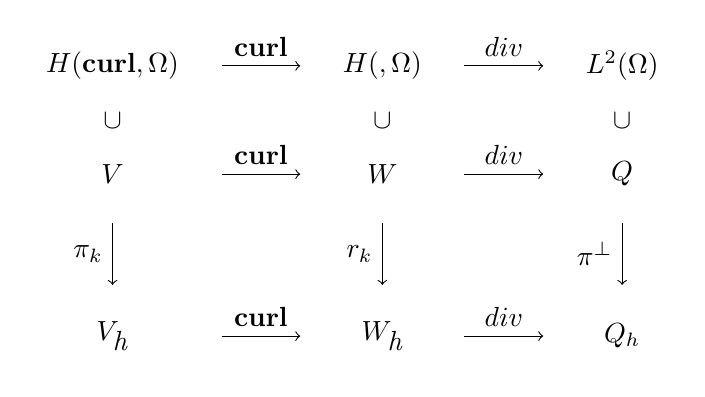
\begin{tikzpicture}[point/.style={circle, inner sep=0pt, minimum size=2pt,fill=red}]
            \matrix[column sep = 1.82mm, row sep = 1.1mm, ampersand replacement = \&] {
             \node {$\text{H}(\textbf{curl},\Omega)$};  
              \& \node (n0) {};
              \& \node      {};
              \& \node (n1) {};
              \& \node (n2) {};
              \& \node {$\text{H}(\Div, \Omega)$}; 
              \& \node (r1c7) {};
              \& \node {};
              \& \node {};
              \& \node (r1c10) {};
              \& \node {$L^2(\Omega)$};\\
             \node (n3) {}; \&\&\&\&\& \node (n5)   {};
              \& \node (r2c7) {};
              \& \node {};
              \& \node {};
              \& \node {};
              \& \node (r2c11) {};\\
             \node (n4) {}; \&\&\&\&\& \node (n6)   {};
              \& \node (r3c7) {};
              \& \node {};
              \& \node {};
              \& \node {};
              \& \node (r3c11) {};\\
             \node (v)  {$V$}; \&\node(fromV){};\&\&\&\node(toW){};\& \node (w) {$W$};
              \& \node (r4c7) {};
              \& \node {};
              \& \node {};
              \& \node (r4c10) {};
              \& \node {$Q$};\\
             \node (n7) {}; \&\&\&\&\& \node (n8)   {};
              \& \node {};
              \& \node {};
              \& \node {};
              \& \node {};
              \& \node (r5c11) {};\\
             \node      {}; \&\&\&\&\& \node        {}; 
              \& \node {};
              \& \node {};
              \& \node {};
              \& \node {};
              \& \node {};\\
             \node      {}; \&\&\&\&\& \node        {}; 
              \& \node {};
              \& \node {};
              \& \node {};
              \& \node {};
              \& \node {};\\
             \node (n11)    {}; \&\&\&\&\& \node (n12) {};
              \& \node {};
              \& \node {};
              \& \node {};
              \& \node {};
              \& \node (r8c11) {};\\
             \node {$V_{\textit{h}} $};                                 
              \& \node (n13) {};
              \& \node       {};
              \& \node (n14) {};
              \& \node (n15) {};
              \& \node {$W_{\textit{h}} $}; 
              \& \node (r9c7) {};
              \& \node {};
              \& \node {};
              \& \node (r9c10) {};
              \& \node {$Q_h$};\\
             };
            \draw[->] (n0) to node[above] {$\textbf{curl}$} (n2); 
            \draw[->] (fromV) to node[above] {$\textbf{curl}$} (toW); 
            \draw[white] (n3) to node {{\color{black}$\cup$}} (n4);
            \draw[white] (n5) to node {{\color{black}$\cup$}} (n6);
            \draw[->] (n7) to node[left] {$\pi_k$} (n11); 
            \draw[->] (n8) to node[left] {$\boldsymbol{r}_k$} (n12); 
            \draw[->] (n13) to node[above] {$\textbf{curl}$} (n15); 
            \draw[->] (r1c7) to node[above] {$\text{div}$} (r1c10);
            \draw[->] (r4c7) to node[above] {$\text{div}$} (r4c10);
            \draw[->] (r9c7) to node[above] {$\text{div}$} (r9c10);
            %\draw[white] (r2c7) to node {{\color{black}$\cup$}} (r3c7);
            \draw[white] (r2c11) to node {{\color{black}$\cup$}} (r3c11);
            \draw[->] (r5c11) to node[left] {$\pi^{\perp}$} (r8c11);
        \end{tikzpicture}
    \end{center}

% subsection definition_of_the_h_div_element (end)

El sigte lema, hacerlo una vez para edge
y una vez para face, para un cierto poliedro, y decir que vale 
la misma cuenta en los otros. Ver (3.79) (3.80) en monk: transf.
de normales y tangentes.\\\\
remite a transform entre prismas etc ... de preliminares
\begin{lemma} The edge element interpolators satisfy
\begin{IEEEeqnarray}{rCl}\label{piTransformado}
    \wku(\hat{\bx}) & = & M^{t} \bw_k\bu(F(\hat{\bx})).
\end{IEEEeqnarray}
{\color{BrickRed} > lo probamos?}
\end{lemma}

% subsection transformaciones_entre_prismas (end)